\documentclass{article}
\setlength{\pdfpagewidth}{8.5in}
\setlength{\pdfpageheight}{11in}
\usepackage{booktabs}
\usepackage{graphicx}
\usepackage[utf8]{inputenc}
\usepackage{fancyvrb}
\usepackage{pgfplots}

\begin{document}

% Use an empty page style for the title and abstract
\pagestyle{empty}

% =====
% Title
% =====
\title{Hardware-Accelerated Rendering of Intersecting Volumes using Boolean Operations}
\author{Andrew Brown \and Joe Geigel}
\date{\small{Rochester Institute of Technology}}
\maketitle

% ========
% Abstract
% ========
\begin{abstract}
Rendering intersecting volumes is problematic because the renderer must
alternate between sampling from each volume to achieve the correct blending.
Methods for rendering an arbitrary number of intersecting volumes using hardware
acceleration have been developed, but they generally require a large amount of
geometry to be created every frame.  This paper investigates whether using
Boolean operations are faster in the simple case where two axis-aligned volumes
intersect.  Although viable options it is shown that two new methods are no
faster than the traditional slicing method.
\end{abstract}

% Switch back to a plain page style for the rest of the paper
\pagestyle{plain}

% ============
% Introduction
% ============
\section{Introduction}

For many years the computing community has created software to visualize data
from medical and scientific equipment.  Normally the data is returned as a
three-dimensional grid of values.  This grid is called a volume, and the
individual values are named voxels, similar to how the elements of a picture are
called pixels.

Volumes produced by such equipment often become quite large, and at first
computers had a difficult time displaying the data in real time.  Early work in
the field thus focused on ways to speed up the process while still maintaining
the highest image quality possible.  In fact, a handful of different methods
with their own unique alterations were tried in the hopes of delivering better
images at a higher frame rate.  In addition, some initial attempts were made at
providing users with better information by simultaneously displaying multiple
volumes in order to place data in its appropriate context.

Of course, as years passed, new technologies developed and it was not long
before high-level, programmable shading languages enabled researchers to utilize
the significant processing power of the main processor on video cards, commonly
called the graphics processing unit, or GPU.  Extremely proficient at performing
similar operations on a large amount of data, GPUs accelerated volume
visualization software tremendously.  Hardware-accelerated implementations of
both the classic slicing method and the high-quality ray-casting method were
developed quickly for single volumes.

With much of the original performance concerns alleviated, and more and more
data being collected from several different sources, researchers are again
looking at ways to effectively display multiple volumes simultaneously.  A few
different methods have been developed for rendering an arbitrary number of
volumes using hardware acceleration, but they can be problematic to implement,
rely on general-purpose GPU programming, or both.

For those reasons, in this paper we examine techniques for rending two volumes
using simple boolean operations.  Although limited, we hope the techniques
presented will be more approachable to software engineers faced with
implementing such technologies, and could help direct future efforts in volume
rendering.

The rest of the paper begins with background information and a more thorough
discussion of previous work in the field.  It then moves on to technologies
available for GPU programming.  Finally, a detailed plan of our proposed work
and its projected implementation is given.

% ==========
% Background
% ==========
\section{Background}

Understanding the techniques presented in this paper is heavily dependent on
knowing some key concepts of how a video card renders three-dimensional objects
by use of a rendering pipeline.  This pipeline is very similar to an assembly
line, where data elements are passed from stage to stage and no element stays in
a stage any longer than it needs to.  It is this unique structure that gives the
video card its speed, since operations are optimized to be performed on a large
amount of data at the same time.

To get the pipeline started, the application feeds vertices to the video card’s
first stage.  So the video card knows which vertices are connected, the
application also provides binding information describing which vertices make up
which polygons.  At this point, the video card’s first stage begins constructing
the polygons and performs some preparatory operations on the vertices, such as
calculating the normal vectors used for illumination and assigning texture
coordinates.  As soon as a polygon is finished, it is immediately passed onto
the next stage, which begins rasterizing the polygons into temporary pixels
called fragments.  The fragments are passed along to the last stage, which
shades the them, decides which ones to discard, and displays those that remain
as pixels.

With the advent of programmable pipelines, developers can now replace some of
the fixed functionality of the pipeline with special programs, called shaders,
that execute custom code, in some cases even making the pipeline do things it
was not designed to do.  The first part of the pipeline that can be replaced is
at the beginning where vertices are prepared for the following stages.  These
shaders are called vertex shaders since they operate on the vertices themselves.
Vertex shaders are normally used to change the position of the vertex, alter its
texture coordinates, or perhaps modify its normal vector.  The second part of
the pipeline that can be replaced is towards the end, where fragments are being
shaded.  Fragment shaders generally change the color of the object or how it is
illuminated.  Many times they look up values stored in textures, which are
generally one, two, or three dimensional images.

Since there are always many fragments generated in rendering an image, designers
have devoted much of the hardware to processing them.  Therefore fragment
shaders are traditionally used to perform the bulk of the work in any
application using a shading language for hardware acceleration.  Because they
are used so much, it is important to note that a fragment’s location is
generally given in normalized texture coordinates.  These coordinates range from
0.0 to 1.0 according to the bounds of the polygon, with 0.0 being one extreme
and 1.0 being the other.

% =============
% Previous Work
% =============
\section{Previous Work}

\subsection{Overview}

The first major breakthrough in volume rendering came with \cite{Levoy88}.
Previous techniques tried to use actual geometry to approximate the surfaces of
volumetric data.  A major problem with these approaches was determining whether
parts of the volume were actually part of a surface or not.  Instead of fitting
geometry to the volume, Levoy’s method samples the volume directly and uses the
resulting vertices to texture a series of polygons aligned with the viewing
direction.  Commonly referred to as slicing, this method was a significant
improvement in accuracy.  Although over twenty years old, sampling the volume
directly has remained the basis for most volume rendering techniques today and
has been termed Direct Volume Rendering.

Levoy made another significant contribution two years later with a paper
\cite{Levoy90} describing Direct Volume Rendering using ray-casting.  Because
many times volumes have large spaces that do not make a difference in the final
image, Levoy focused on having rays skip those spaces by consulting a
hierarchical space division technique known as an octree.  This method has
become known as Empty Space Skipping and is still very important to ray-casting
implementations.

Not long after, Danskin and Hanrahan \cite{Danskin92} improved on Levoy’s work
by integrating another form of acceleration into ray-casting.  Called early ray
termination, the procedure stops the ray if its opacity ever reaches a level
where further samples will not change the final image.  Fairly straightforward
and easy to implement, early ray termination is a staple for most applications.

In 1994 Cullip and Neumann \cite{Cullip94} took another look at the slicing
method.  They primarily compared different methods for orienting the textured
polygons of the slicing method.  The first method oriented the polygons with the
object-space axes.  The other aligned them in image-space.  The former requires
reorienting the polygons as the viewport changes, but the latter must be clipped
to object space requiring a transformation with the inverse viewing matrix.  It
was further suggested that the image-space method would require more passes.
Another important contribution was using a progressive rendering algorithm while
the user is rotating the scene.

Jumping ahead, in \cite{Leu99} Leu and Chen developed a practical platform for
rendering multiple volumes featuring a two-layer approach that separated volume
data from instances of that data.  Consideration for memory management in the
case that all the data did not fit into memory was made, although intersecting
volumes were not considered.

A key source for vital information concerning volume ray-casting with high-level
programmable shading languages came with \cite{Kruger03}.  Kruger demonstrated
that an implementation using fragment shaders and featuring early ray
termination can achieve significant performance gains.  Much of the credit was
given to new features of graphics APIs, including accessing multiple textures,
rendering to arbitrary textures, and replacing depth buffer values.  His
implementation with early-ray termination and ray-casting generally outperformed
other methods by a factor of three and normal ray-casting by a factor of four
for most data sets.

A comprehensive review of the slicing method applied to the GPU can be obtained
from \cite{Ikits04}.  Ikits describes the techniques required for creating the
proxy geometry, texturing the slices using NVIDIA’s Cg shading language, and
using the gradient for local and global illumination models.

\cite{Ruijters06} examined bottlenecks in hardware and devised a two-staged
method for balancing between them.  The first stage breaks the volume into
rectangular bricks, getting rid of empty ones and relieving a bottleneck with
texture memory and the memory bus.  The second stage meanwhile helps in
eliminating details that will not be rendered during rasterization.

Recent work in the field has focused on visualizing multiple volumes.  This
ability helps those that view the data to judge the information in context to
other relevant data.

Grimm \cite{Grimm04} presented techniques to render multiple volumes with the
CPU.

In particular Roßler et.\ al.\ \cite{Rossler06} allowed MRI scans of the human
brain to be viewed simultaneously with the skull by using the slicing method.
An important feature was being able to manipulate each model, in regards to
clipping and opacity, independently of the other.

Later \cite{Rossler08} rendered multiple volumes using the ray-casting method
developed by Kruger.  Rather than render all the volumes at once, which could
sample a large amount of empty space, his technique splits the scene into
multiple regions and generates shaders dynamically.

Some researchers have moved to using general-purpose technologies like CUDA or
OpenCL to better leverage the GPU for multi-volume rendering.  The
implementation by Kainz et. al. \cite{Kainz09} was slower for simple cases, but could
render more complicated scenes.

\subsection{Slicing}

The classic method for performing volume rendering on the GPU is called slicing.
Slicing uses polygons perpendicular to the viewing direction, called proxy
polygons or slices, to sample the volume at regular intervals.  When the entire
volume has been sampled, the slices are composited together to form the final
image.  Because of its relative simplicity, slicing generally yields the fastest
frame rates of all volume rendering methods.

The first step in slicing is to transform the coordinates of the volume’s
bounding box so that they are in terms of the viewing direction.  This is
necessary because the coordinates of the bounding box are stored relative to
itself, but slicing needs the coordinates after any rotations or translations
have been applied.  Luckily, handling this transformation is as simple as
applying the model-view matrix.

Next, the slices are made by generating planes from the closest z position of
the bounding box to the farthest.  The planes are made at regular intervals
according to the image quality desired.  Each resulting plane is tested for
intersections with each edge of the bounding box using the plane-line
intersection test formula.  Any resulting intersection points that fall within
the bounds of the polygon are then sorted into a clockwise or counterclockwise
direction to form the proxy polygon corresponding to that plane.

Now the slices are ready to sample the volume.  A fragment shader is responsible
for performing this operation, looking up voxels based on the texture
coordinates of fragments generated from rendering the slices.  As long as the
vertices of the slices were given texture coordinates that correspond with how
the volume is indexed, the fragment shader’s job is simple.  Except for some
rounding and interpolation, the texture coordinate of the fragment can be used
to access the volume directly, returning a value for that position.  The value
is fed into a transfer function and the resulting color is blended into the
framebuffer.

\begin{figure}
\centering
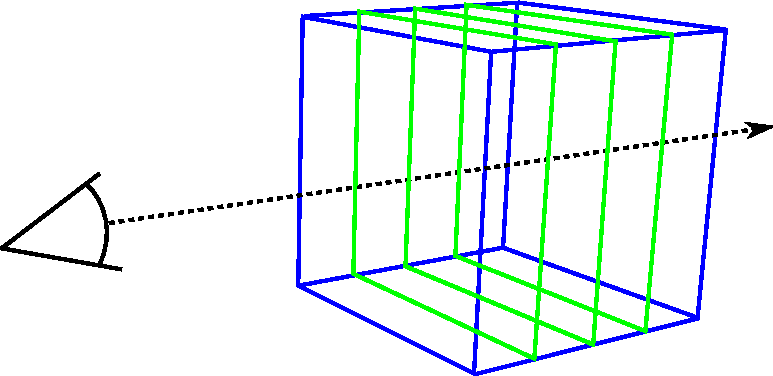
\includegraphics[width=0.8\textwidth]{slicing-aligned.pdf}
\caption{Three slices through aligned volume.}
\label{slicing-aligned}
\end{figure}

\begin{figure}
\centering
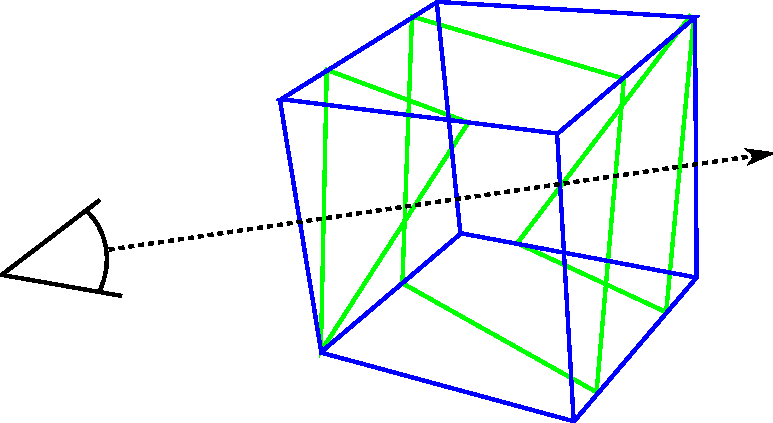
\includegraphics[width=0.8\textwidth]{slicing-rotated.pdf}
\caption{Three slices rotated through volume.}
\label{slicing-rotated}
\end{figure}

Figures \ref{slicing-aligned} and \ref{slicing-rotated} are illustrations
adapted from \cite{Ikits04} showing the process of generating and texturing the
slices.  The first figure shows a trivial example where the volume is aligned
with the viewing direction.  Slices generated are simply rectangles the same
size of the volume.  The volume in the second figure however has been rotated by
the user, and thus the slices are more irregular shapes.

Note that we take the approach of keeping the viewpoint fixed.  Instead of
seeing the viewpoint as rotating around the volume, consider the volume to be
rotating in front of the viewpoint.  We believe this methodology is easier to
understand since the view-space axes are then always aligned with world-space.

\section{Ray Casting}

Ray-casting is an alternate method for performing volume visualization.  Along
with being quite simple and elegant, it is generally considered to produce the
highest-quality images, and has thus become quite popular.  Although usually
slower than slicing, some acceleration methods have been developed that make its
speed quite competitive.

In traditional ray-casting, as in implementations not associated with volume
rendering, rays are projected from the viewpoint through a pixel grid located in
front of the scene.  A ray is created for each pixel in the grid, and each
resulting ray is tested for intersections with every object in the scene.  The
color of the closest intersecting object is then stored as the color for the
corresponding pixel in the grid.  Once all the rays have finished, the values in
the grid are copied to the frame-buffer.  Figure \ref{traditional-ray-casting}
shows an overhead model of the traditional ray-casting process.

\begin{figure}
\centering
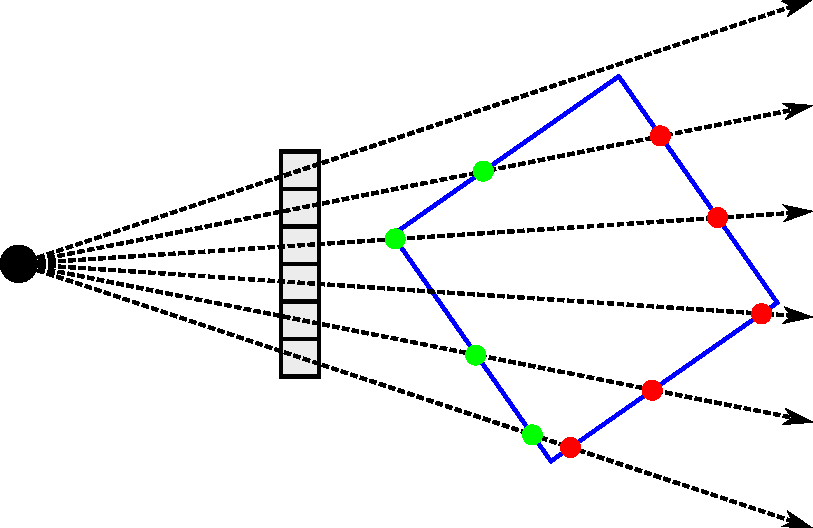
\includegraphics[width=0.8\textwidth]{traditional-ray-casting.pdf}
\caption{Traditional ray-casting with pixel grid.}
\label{traditional-ray-casting}
\end{figure}

To apply ray-casting to volume rendering with a high-level programmable shading
language, \cite{Kruger03} adapted the concept to use fragment shaders on a
volume’s bounding box.  Instead of casting rays through a pixel grid, each
fragment generated by rendering the bounding boxes creates its own ray.  The
rays start at the viewpoint and passes through the fragment’s location.  Any
volumes that intersect the ray are sampled at regular intervals along it by
applying the inverse model view matrix to the points and using them as indices
into the volume.  A transfer function converts the values to colors, and each is
blended into the framebuffer at the fragment’s position.  Figure
\ref{fragment-ray-casting} gives a depiction of the process, with green circles
representing fragments.

\begin{figure}
\centering
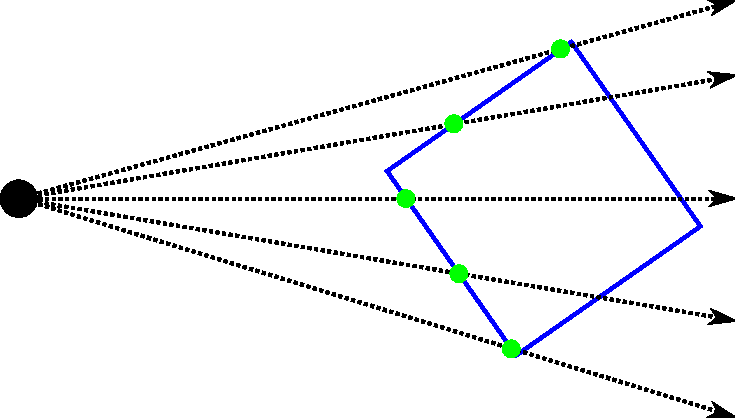
\includegraphics[width=0.8\textwidth]{fragment-ray-casting.pdf}
\caption{Ray-casting by fragments.}
\label{fragment-ray-casting}
\end{figure}

The simplest acceleration technique inherent to ray-casting is early ray
termination, which stops calculation when a certain threshold has been reached
while marching along the ray.  Fairly intuitive, early ray termination works
because if the data has already added up to be opaque, values behind it no
longer make a difference.

Early ray termination is not the only way to accelerate ray-casting. A more
complicated technique is called empty space skipping.  Pioneered by Marc Levoy
in 1990 \cite{Levoy90}, empty space skipping is traditionally done with an
octree.

An octree is a tree data structure used to divide a three-dimensional space,
with each node representing a section of that space.  The first node in the
tree, the root, is the size of the entire space, and as the name implies, it is
broken up into eight smaller sections.  These sections are added as children to
the root node, and then they are split into eight smaller sections themselves.
The process continues until the sections reach a size that the application is
comfortable working with.

With the sizes set, the nodes at the bottom of the tree, called leaf nodes, set
various characteristics based on the objects inside their section of the space.
Nodes in the rest of the tree then use the characteristics of their eight
children nodes to set their own characteristics.  In this way an octree holds
information about the space on many different levels of detail, which an
application can use to intelligently navigate and make decisions about the
space.  Figure \ref{octree} shows the first three levels of an octree.

\begin{figure}
\centering
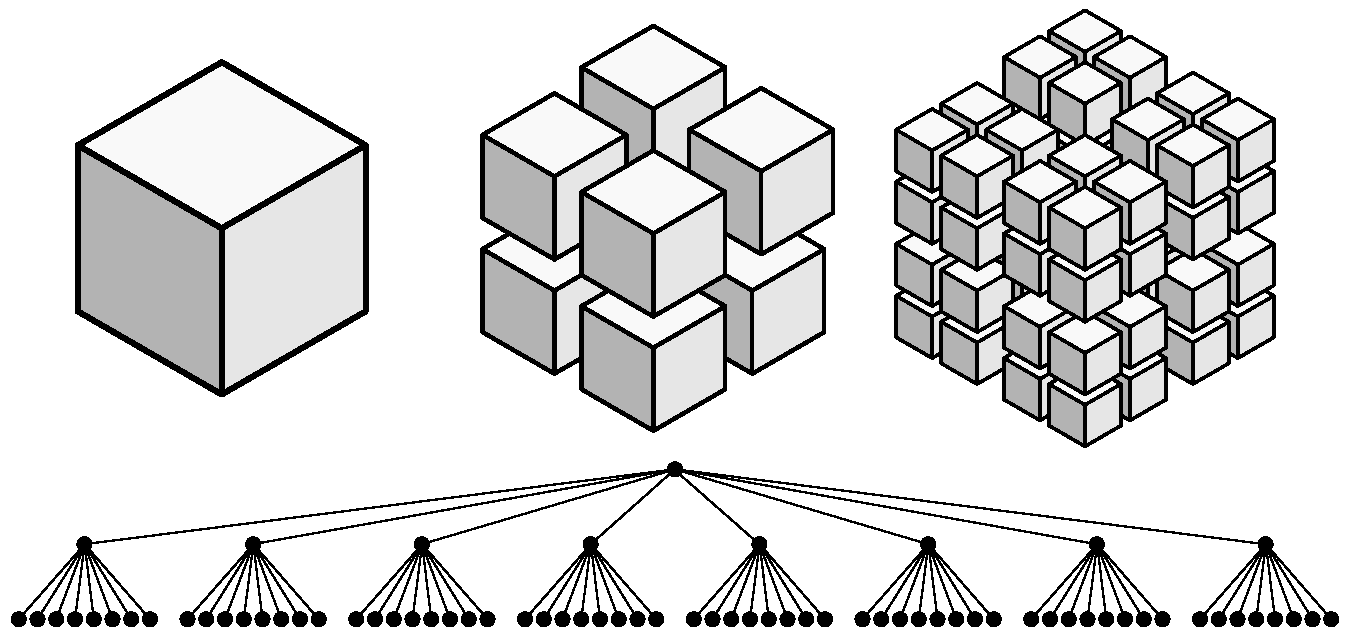
\includegraphics[width=0.9\textwidth]{octree.pdf}
\caption{The first three levels of an octree.}
\label{octree}
\end{figure}

For volume rendering, an octree represents the space of the volume, and its
nodes store whether that section of the space is empty or not.  A leaf node,
which has a width equal to twice the distance between two voxels, is determined
to be empty if all of the eight voxels at its corners are below a certain
threshold.  Larger nodes meanwhile are empty if the eight nodes below them are
all empty.  With an octree of this sort in place, rays can potentially save
themselves a lot of work by checking the nodes in the octree before sampling,
starting with the root and working its way down.  If the ray ever encounters an
empty section, it can skip over all the points along the ray that would fall in
that section.

% ==========
% Approaches
% ==========
\section{Approaches}

We take two different approaches to rendering intersecting volumes using boolean
operations.

The boolean operations involved are AND and XOR.  AND takes the intersection of
two shapes, while XOR, meaning exclusive OR, takes everything but the
intersection.

Both approaches are based on the volume rendering method in \cite{Kruger03}, as
previously mentioned.  To render part of a volume, they first render the texture
coordinates of the back faces of that part to a texture.  Then the front faces
of that part are rendered with a shader that uses the previously-stored texture
coordinates to form a ray through the volume.  The ray then samples the volume
at regular intervals.

In addition, both approaches use multiple passes.  To blend the samples
correctly between passes, each pass must start with the results of the previous
pass.  The results of all the passes cannot be simply blended together
afterwards.

\subsection{Boolean AND with Depth Buffer Masking}

The first approach uses a Boolean AND operation combined with depth-buffer
masking.  The basic idea is render the part of the volume directly behind the
intersection, render the intersection itself, and then render the part of the
volume directly in front of the intersection.  Finally the area of the
intersection is masked off and everything else is drawn depth-sorted with
blending enabled.

\begin{figure}
\centering
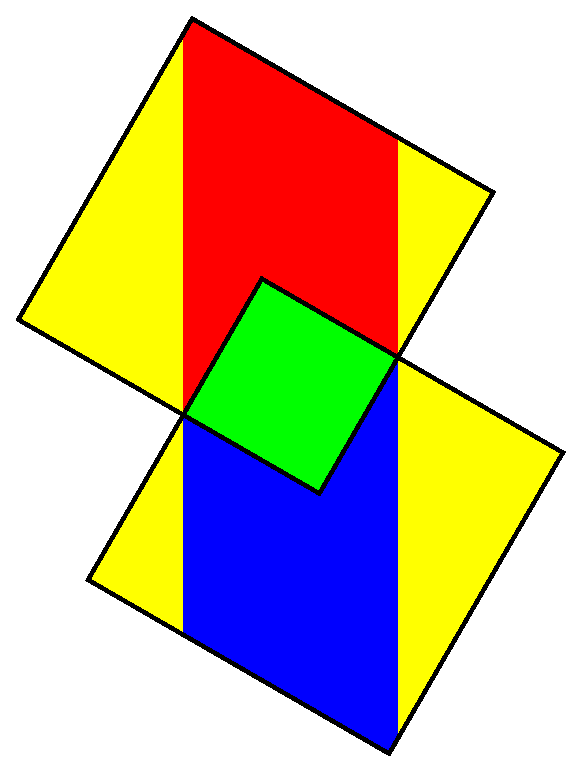
\includegraphics[width=0.8\textwidth]{boolean-and.pdf}
\caption{
Top-down view of rendering intersecting volumes using the Boolean AND with depth
buffer masking approach.  First the part of the volume directly behind the
intersection, colored red, is rendered.  Next the intersection, colored green,
is rendered.  Then the the part of the volume directly in front of the
intersection, colored blue, is rendered.  Finally the depth buffer is masked off
using the Boolean AND so that when the cubes are rendered again, only the parts
colored yellow are rendered.
}
\label{boolean-and}
\end{figure}

It is mostly GPU-based, only requiring that the Boolean operation be performed
on the CPU.  While there is relatively less work on the CPU, it does require a
significant amount of passes.

The first step in this approach is to bind all the textures.  There are two for
the volumes, two for storing the texture coordinates of the back faces of the
cubes, and one for storing results between passes.  The last three textures will
be used with external framebuffers, so they should have a width and height at
least as big as the window.

\begin{enumerate}
  \item Bind volume textures
  \item Bind textures to store texture coordinates
  \item Bind texture to store results
\end{enumerate}

Next the part of the volume behind the intersection is rendered into the results
texture.  To get just that part the back faces of the Boolean AND are used
instead of the front faces of the cube.

\begin{enumerate}
  \item Cull front faces
  \item Bind framebuffer with coordinates texture
  \item Activate shader program for rendering texture coordinates
  \item Draw cube behind intersection
  \item Bind framebuffer with results texture
  \item Activate shader program for rendering a volume
  \item Draw Boolean AND of cubes
\end{enumerate}

From there the intersection itself is rendered.  Because the intersection needs
to alternate between samples from both volumes, we have to render the back face
coordinates into two different textures, and then make them both available to
the shader program that renders the intersection.

\begin{enumerate}
  \item Cull front faces
  \item Bind framebuffer with first coordinates texture
  \item Activate shader program for rendering primary texture coordinates
  \item Draw Boolean AND of cubes
  \item Bind framebuffer with second coordinates texture
  \item Activate shader program for rendering secondary texture coordinates
  \item Draw Boolean AND of cubes
  \item Cull back faces
  \item Bind framebuffer with results texture
  \item Activate shader program for rendering volume
  \item Draw Boolean AND of cubes
\end{enumerate}

After that the part of the volume in front of the intersection is rendered to
the results texture.

\begin{enumerate}
  \item Cull back faces
  \item Bind framebuffer with coordinates texture
  \item Activate shader program for rendering primary texture coordinates
  \item Draw cube in front of intersection
  \item Bind framebuffer with results texture
  \item Activate shader program for rendering volume
  \item Draw Boolean AND of cubes
  \item Mask off depth buffer
\end{enumerate}

The area of the screen with the intersection should be masked off so that
nothing else in that area will be rendered.

\begin{enumerate}
  \item Activate shader program for setting depth to zero
  \item Draw Boolean AND of cubes
\end{enumerate}

Finally we render the two volumes again depth-sorted with blending enabled and
the depth function set to \emph{LESS}.  Since on the previous step we masked off
the area of the screen with the intersection, the fragments in those parts will
just be discarded.  In fact, on most modern video cards they will not even be
processed by the fragment shader at all because of early Z-kill.

\begin{enumerate}
  \item Enable blending
  \item Set depth function to \emph{LESS}
  \item Bind framebuffer with coordinates texture
  \item Cull front faces
  \item Activate shader program for rendering primary texture coordinates
  \item Draw cube behind intersection
  \item Cull back faces
  \item Activate shader program for rendering volumes
  \item Draw cube behind intersection
  \item Repeat for cube in front of intersection
\end{enumerate}

\subsection{Boolean AND with Boolean XOR}

The second approach uses a Boolean AND operation together with a Boolean XOR.
Here the idea is to break up both volumes into pieces around the intersection.
All the pieces behind the intersection are rendered first, then the intersection
itself, and then all the pieces in front of the intersection.

\begin{figure}
\centering
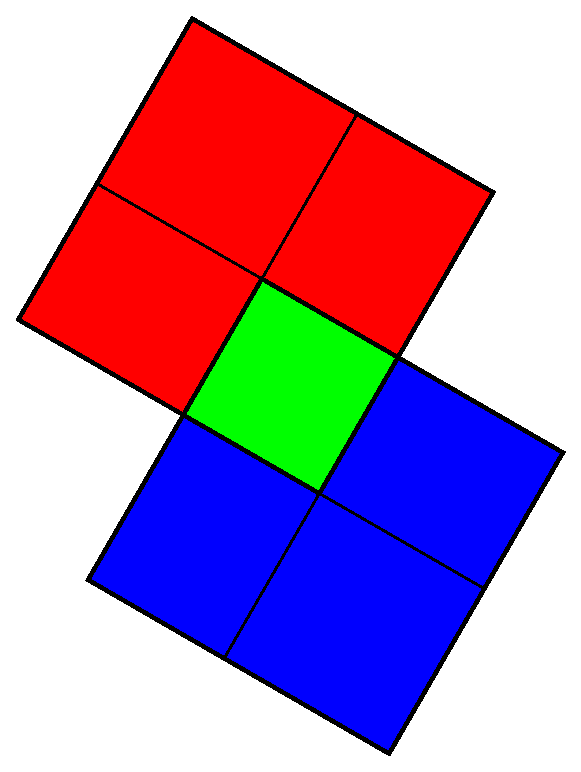
\includegraphics[width=0.8\textwidth]{boolean-xor.pdf}
\caption{
Top-down view of rendering intersecting volumes using the Boolean AND with
Boolean XOR approach.  First the pieces behind the intersection, colored red,
are rendered.  Next the intersection, colored green, is rendered.  Then the
pieces in front of the intersection, colored blue, are rendered.  A final pass
renders the results to the screen.
}
\label{boolean-xor}
\end{figure}

Like the first approach, the first step is to set up the textures.  There are
two textures for the volumes, two to store the texture coordinates of the back
faces, and one to hold results between passes.  The textures to store the
texture coordinates and results between passes will be used with external
framebuffer objects, and should thus be at least as big as the window.

\begin{enumerate}
  \item Bind volume textures
  \item Bind textures to store texture coordinates
  \item Bind texture to store results
\end{enumerate}

Storage should also be created to act as a depth buffer for some passes.  Since
we do not need to read from it, it can just be a \emph{renderbuffer}.  It also
needs to be at least as big as the window.

\begin{enumerate}
  \item Create depth renderbuffer
\end{enumerate}

Next the results texture should be cleared.

\begin{enumerate}
  \item Bind framebuffer with results texture
  \item Clear color
\end{enumerate}

Then the pieces behind the intersection should be used to render the volumes to
the results texture.  Because there may be multiple pieces behind the
intersection and we only want the texture coordinates of the faces that are
farthest back, we first clear the depth buffer to zero and set the depth
function to \emph{GREATER}.  Once we have those coordinates stored, we do the
opposite by clearing the depth buffer to one and setting the depth function back
to \emph{LESS}.  That way we render using the faces that are farthest forward.

\begin{enumerate}
  \item Bind framebuffer with coordinates texture and depth renderbuffer
  \item Clear depth to zero
  \item Set depth function to \emph{GREATER}
  \item Cull front faces
  \item Activate shader program for rendering primary texture coordinates
  \item Draw Boolean XOR with pieces behind intersection
  \item Bind framebuffer with results texture and depth renderbuffer
  \item Clear depth to one
  \item Set depth function to \emph{LESS}
  \item Cull back faces
  \item Activate shader program for rendering volumes
  \item Draw Boolean XOR with pieces behind intersection
\end{enumerate}

Following our pattern, we now render the intersection itself.  Notice we do not
need a depth buffer for this pass, although we do need to make sure both sets of
texture coordinates are stored and are available when we render the
intersection.

\begin{enumerate}
  \item Cull front faces
  \item Bind framebuffer with first coordinates texture
  \item Activate shader program for rendering primary texture coordinates
  \item Draw Boolean AND of cubes
  \item Bind framebuffer with second coordinates texture
  \item Activate shader program for rendering secondary texture coordinates
  \item Draw Boolean AND of cubes
  \item Cull back faces
  \item Bind framebuffer with results texture
  \item Activate shader program for rendering volumes
  \item Draw Boolean AND of cubes
\end{enumerate}

Next we render any pieces of the cube in front of the intersection to the
results texture.  Similar to the first pass, we use the depth buffer to make
sure we only take the texture coordinates of the faces we want.

\begin{enumerate}
  \item Bind framebuffer with coordinates texture and depth renderbuffer
  \item Cull front faces
  \item Set depth function to \emph{GREATER}
  \item Clear depth buffer to zero
  \item Activate shader program for rendering primary texture coordinates
  \item Draw Boolean XOR with pieces in front of intersection
  \item Bind framebuffer with results texture and depth renderbuffer
  \item Cull back faces
  \item Set depth function to \emph{LESS}
  \item Activate shader program for rendering volumes
  \item Draw Boolean XOR with pieces in front of intersection
\end{enumerate}

Finally we render the results to the screen by drawing both cubes again.  The
shader program for this final pass just outputs whatever is in the results
texture.  We need this final pass because depending on how the scene is laid out
there may not be any pieces behind or in front of the intersection, meaning the
first and third passes may not be run.

\begin{enumerate}
  \item Activate shader for rendering results
  \item Render both cubes
\end{enumerate}

It is mostly CPU-based, since it requires both Boolean operations to be done on
the CPU.  The extra work on the CPU results in less rendering passes, however.
The pseudocode for the approach is shown below.

% ==============
% Implementation
% ==============
\section{Implementation}

The two approaches were implemented using OpenGL with C++.  To ensure results
are relevant to current and future applications, we used only the core profile
of OpenGL 3.  In other words, no deprecated functionality from OpenGL 2 was
used.  Furthermore, because OpenGL 4 is a superset of the OpenGL 3 core profile,
the implementation will easily work with that as well.

To facilitate the process, a handful of general-purpose graphics libraries were
developed.

At the lowest levels are a simple 3D mathematics library and a library providing
thin C++ wrappers around the components already in OpenGL.  Above that, another
library provides additional utilities for working with OpenGL, including one for
loading volumetric data as a texture, and another for rendering text.

At the highest level is a library named {\em RapidGL} providing a simple render
graph that can be used to rapidly prototype OpenGL applications.  Similar to
SVG, or Scalable Vector Graphics, the render graph can be written in XML so
scenes can easily be saved, reloaded, and shared.  In addition, users are free
to experiment with their scenes without ever recompiling the application.

Core to RapidGL is the {\tt Node} class.  Nodes can override the {\tt visit}
method to perform actions when the scene is traversed.  Most implementations
perform any setup which requires other nodes the first time they are visited.
For example, many nodes check for ancestors with specific types or search the
scene for nodes with a specific ID.  Nodes can also register themselves as {\em
listeners} of other nodes by implementing the {\tt NodeListener} interface and
passing a pointer to the node's {\tt addNodeListener} method.

The XML below shows how the second pass of the first approach is rendered.
Notice that the render graph supports basic instancing through the {\em group}
and {\em instance} nodes.  When an instance node is visited, it simply traverses
the group it points to.  Complex behavior can be achieved with nested groups.

\begin{Verbatim}[fontsize=\small]
  <cull faces="front" />
  <framebuffer>
    <attachment usage="color" link="coords-texture-1" />
    <use program="primary-coords-program">
      <group id="intersection-group">
        <booleanAnd of="cube-1 cube-2" />
      </group>
    </use>
  </framebuffer>
  <framebuffer>
    <attachment usage="color" link="coords-texture-2" />
    <use program="secondary-coords-program">
      <instance of="intersection-group" />
    </use>
  </framebuffer>
  <cull faces="back" />
  <framebuffer>
    <attachment usage="color" link="results-texture" />
    <use program="second-pass-program">
      <uniform name="CoordsTexture1" link="coords-texture-1" />
      <uniform name="CoordsTexture2" link="coords-texture-2" />
      <uniform name="VolumeTexture1" link="volume-texture-1" />
      <uniform name="VolumeTexture2" link="volume-texture-2" />
      <uniform name="MVPMatrix" usage="modelviewprojection" />
      <instance of="intersection-group" />
    </use>
  </framebuffer>
\end{Verbatim}

The Boolean operations required by the two approaches were implemented as two
separate nodes.  Currently both nodes take two cubes, which are assumed to be
axis-aligned.  {\tt BooleanAndNode} finds the intersection of the two cubes by
finding the minimums and maximums of the cubes in world space.  {\tt
BooleanXorNode} does the same, but then uses a variation of the well-known
Sutherland-Hodgman polyline-clipping algorithm to break up the cubes into pieces
around the intersection.  Both nodes use the {\tt NodeListener} interface to
only update their geometry when the cubes move.

All of the libraries can be compiled as shared libraries using GCC on Linux and
Mac OS X.  Some libraries require {\em Poco} for text and XML utilities.  {\em
GLFW} and {\em CppUnit} are also required by some libraries for unit testing.

From there an application was created to view RapidGL scenes.  Users can
rotate the camera around a scene, as well as select objects and drag them.  The
application shows the current frame rate so the performance of a scene can be
evaluated.

\begin{figure}
\centering
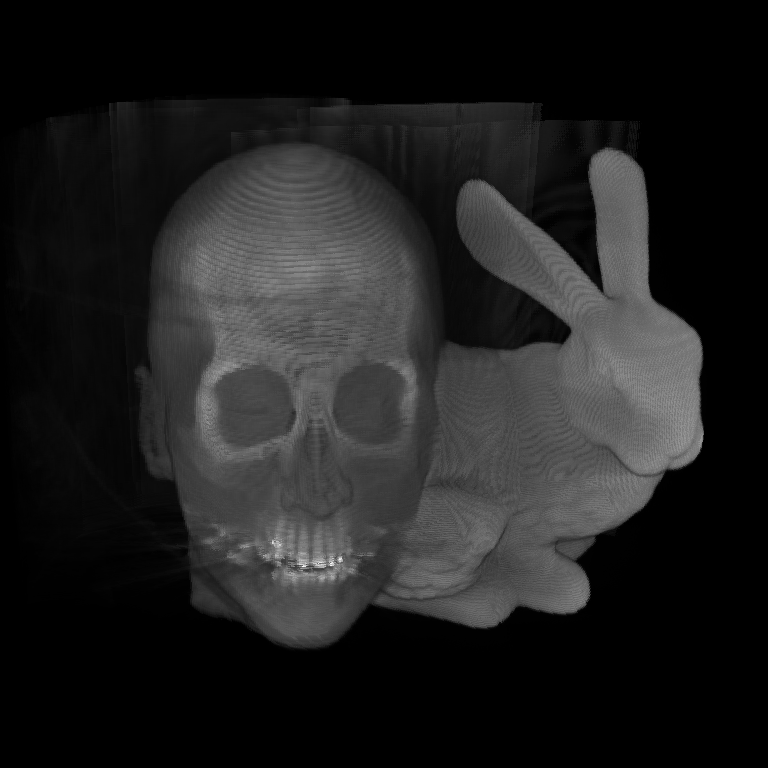
\includegraphics[width=0.95\textwidth]{boolean-and-screenshot-2.png}
\caption{Screenshot of Boolean AND.}
\end{figure}

\begin{figure}
\centering
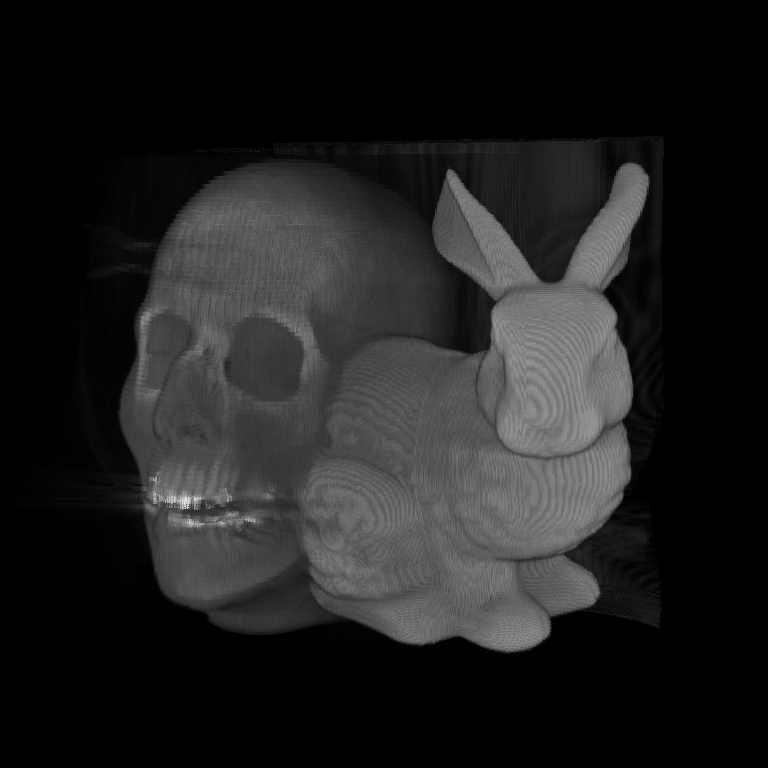
\includegraphics[width=0.95\textwidth]{boolean-xor-screenshot-2.png}
\caption{Screenshot of Boolean XOR.}
\end{figure}

% ==========
% Evaluation
% ==========
\section{Evaluation}

The two approaches to rendering intersecting volumes using boolean operations
were evaluated using different criteria.

Because volume visualization is used in the scientific and medical communities
to aid in making important decisions, an approach that does not handle all cases
will likely not be appropriate for widespread usage.  With that in mind, the
accuracy of each approach was judged by looking for edge cases with visual
artifacts.

Unfortunately the Boolean XOR approach may show some visual artifacts from
certain angles.  Figure \ref{boolean-xor-with-artifact} shows an example of the
artifact.  This occurs because when two pieces have the same depth value, due to
perspective one of the pieces may actually appear behind the other, as
illustrated in figure \ref{pieces-in-perspective}.  In the future, this issue
may be solved by using the distance from the camera to sort rather than the
actual depth.

\begin{figure}
\centering
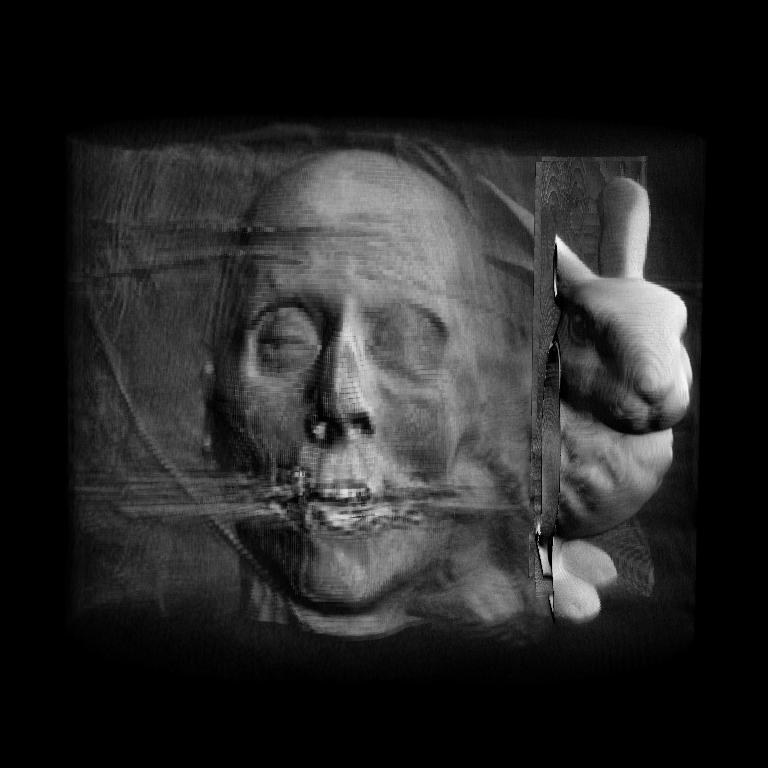
\includegraphics[width=0.95\textwidth]{boolean-xor-screenshot-3.png}
\caption{Screenshot of Boolean XOR with visual artifact.}
\label{boolean-xor-with-artifact}
\end{figure}

\begin{figure}
\centering
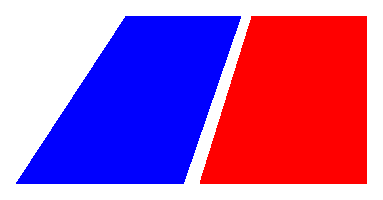
\includegraphics[width=0.95\textwidth]{pieces-in-perspective.pdf}
\caption{Top-down view of two pieces in perspective.  Notice how even though
both pieces have the same depth, a small sliver of the blue piece on the left
ends up being rendered behind the red piece on the right.}
\label{pieces-in-perspective}
\end{figure}

The performance of each approach was measured by using a simple frame counter
showing the number of frames rendered in the previous second.  Multiple camera
angles and scene configurations were tried in order to expose strong and weak
points of the approaches.  The tests were run on at least three different
machines with a variety of operating systems (Linux, Mac OS X) and video cards
(ATI, NVIDIA).  Table \ref{performance-table} shows the results.

\begin{table}
  \centering
  \begin{tabular}{ l l l }
    \toprule
    Approach & Macbook & Desktop \\
    \midrule
    Boolean AND with masking & 22 & 13 \\
    Boolean AND with XOR & 24 & 13 \\
    Slicing & 6 & 18 \\
    Optimized Slicing & 25 & 15 \\
    \bottomrule
  \end{tabular}
  \caption{Performance measurements}
  \label{performance-table}
\end{table}

Furthermore, a variety of sampling rates were used to determine how each
approach scales as the number of samples taken increases.  Figure
\ref{macbook-performance-chart} shows how the methods scale on a 2.2 GHz Intel
Core i7 Macbook Pro with an AMD Radeon HD 6750M video card.  Likewise figure
\ref{desktop-performance-chart} does so for an older 3.0 GHz Intel Pentium 4
Linux desktop with an NVIDIA GeForce 8500 GT video card.

As a baseline the Boolean-based approaches were compared to the existing
view-aligned slicing method from previous work by developing a simple prototype.
Since the slicing method requires significantly more state changes when the
volumes are side-by-side as opposed to when one is in front of the other, it was
particularly important with this method that performance measurements were taken
from a variety of perspectives.

In addition, a variation of the slicing method that was optimized for two
volumes was created.  Basically rather than using uniform variables to switch
textures as would normally be done, the optimized variation stores the texture
with each vertex instead.  While it requires a fairly significant amount of
extra storage, using vertex attributes allows all the slices to be transferred
to the card at once.  The result is a considerable performance boost, similar to
how it is generally faster to transfer one large file across a network then many
small ones.

As shown both Boolean-based approaches outperformed the traditional slicing
method, but were in turn bested by the optimized slicing method.  It should be
noted that the frame rates for the optimized slicing method are the worst case,
and in average it performed even better, around forty frames per second.

Judging from the numbers, it appears that the multiple passes of the
Boolean-based approaches create too much overhead compared to the optimized
slicing method.  The optimized slicing method also has a very simple fragment
shader which may keep it from being fragment-bound.

\begin{figure}
\centering
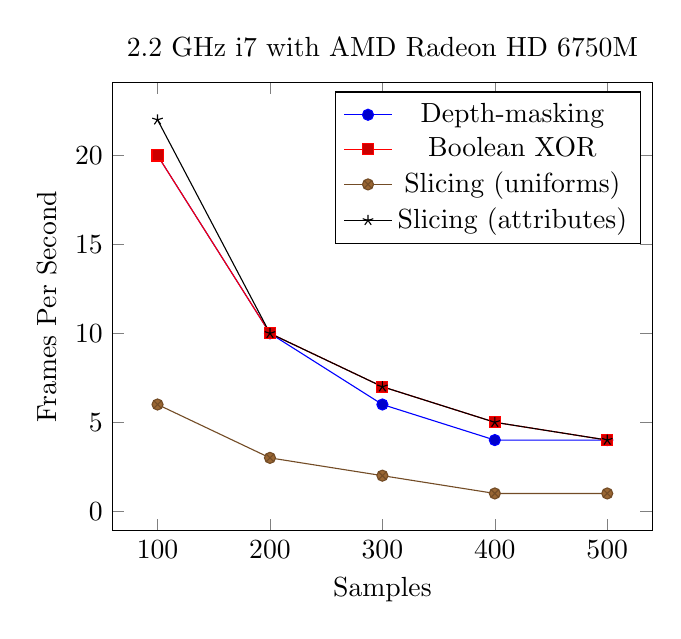
\begin{tikzpicture}
\begin{axis}[
    title=2.2 GHz i7 with AMD Radeon HD 6750M,
    xlabel=Samples,
    ylabel=Frames Per Second]
\addplot coordinates {
  (100, 20)
  (200, 10)
  (300, 6)
  (400, 4)
  (500, 4)
};
\addlegendentry{Depth-masking}
\addplot coordinates {
  (100, 20)
  (200, 10)
  (300, 7)
  (400, 5)
  (500, 4)
};
\addlegendentry{Boolean XOR}
\addplot coordinates {
  (100, 6)
  (200, 3)
  (300, 2)
  (400, 1)
  (500, 1)
};
\addlegendentry{Slicing (uniforms)}
\addplot coordinates {
  (100, 22)
  (200, 10)
  (300, 7)
  (400, 5)
  (500, 4)
};
\addlegendentry{Slicing (attributes)}
\end{axis}
\end{tikzpicture}
\caption{
Chart showing performance measurements as number of samples varies.  The slicing
with attributes, boolean XOR, and depth-masking methods are all about the same,
while the slicing with uniforms method lags behind considerably.
}
\label{macbook-performance-chart}
\end{figure}

\begin{figure}
\centering
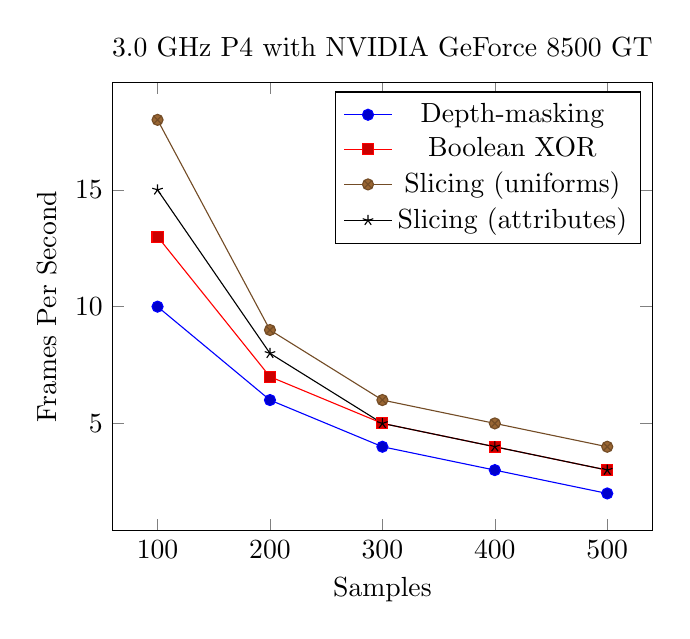
\begin{tikzpicture}
\begin{axis}[
    title=3.0 GHz P4 with NVIDIA GeForce 8500 GT,
    xlabel=Samples,
    ylabel=Frames Per Second]
\addplot coordinates {
  (100, 10)
  (200, 6)
  (300, 4)
  (400, 3)
  (500, 2)
};
\addlegendentry{Depth-masking}
\addplot coordinates {
  (100, 13)
  (200, 7)
  (300, 5)
  (400, 4)
  (500, 3)
};
\addlegendentry{Boolean XOR}
\addplot coordinates {
  (100, 18)
  (200, 9)
  (300, 6)
  (400, 5)
  (500, 4)
};
\addlegendentry{Slicing (uniforms)}
\addplot coordinates {
  (100, 15)
  (200, 8)
  (300, 5)
  (400, 4)
  (500, 3)
};
\addlegendentry{Slicing (attributes)}
\end{axis}
\end{tikzpicture}
\caption{
Chart showing performance measurements as number of samples varies.  Here the
slicing with uniforms method is fastest, followed by the slicing with attributes
method, and the Boolean XOR method.  The depth-masking method is slowest.
}
\label{desktop-performance-chart}
\end{figure}

Altogether, although the Boolean-based approaches outperform the un-optimized
slicing method, it is recommended that the traditional slicing method with the
optimizations described be used.  The optimized slicing method is not only
faster, but it supports volumes of any orientation.  Furthermore, the optimized
method should scale to more volumes relatively easily.

However, it is hoped that the lessons learned in this paper, namely that the
overhead incurred by multi-pass algorithms may outweigh the cost of streaming
geometry in other algorithms, will prove valuable to future endeavors in both
volume rendering and graphics in general.

% ============
% Bibliography
% ============

\newpage
\bibliographystyle{alpha}
\bibliography{paper.bib}

\end{document}
